% Chapter 3

\chapter{The HyperManager} 
\label{chap:hyper} 

\epigraph{\textit{“Design is a funny word. Some people think design means how it looks. 
                             But of course, if you dig deeper, it's really how it works."}}{Steve Jobs}


 This chapter discusses the formal specification and verification by model-checking 
 of a reconfigurable monitoring application --- \thehm. The \pnets\ formalism is 
 employed as a means to describe its behaviour and dynamic topology. 
 
	Section \ref{sub:thehm} presents \textsc{The HyperManager} application. The overall
	methodology employed for this case study is discussed in Section \ref{sec:methodology}.
	Section \ref{sec:spec} and Section \ref{sec:reconfig} detail the formalization aspects and
	proven properties. Final remarks
	are discussed in Section \ref{sec:hyperremarks}
 
	The results discussed in this chapter were partially presented as an industrial case study at the Jiangxi Normal University, China, for the $10^{th}$ \textit{International Symposium on Formal Aspects of Component Software} \cite{GASHENMAD:FACS13}.


\minitoc

\lhead{Chapter 3. \emph{The HyperManager}} % This is for the header on each page - perhaps a shortened title

%----------------------------------------------------------------------------------------


  As discussed in Section \ref{sec:spinnaker}, \spinnaker\ is a French collaborative
  project between INRIA and several academic and industrial partners whose overall goal
  aims at promoting the widespread adoption of \ac{RFID}-based technology. In this context,
  our contribution came with the design and implementation of a non-intrusive, flexible and 
  reliable solution that can integrate itself with other already deployed systems. 
  	
	Specifically, we developed the \thehm, a general purpose monitoring
	application with autonomic features. This was built using GCM/ProActive. For the purposes
	of this project, it had the goal to monitor the \ac{ECW}\footnote{\url{http://www.tagsysrfid.com/Products-Services/RFID-Middleware}}  
	framework in a loosely coupled manner.
	
%retail and healthcare sectors.	
	
	For the sake of clarity let us describe one of the real life scenarios faced in a industrial 
	context. An hotel needs to keep track of 
	their bed sheets life-cycle. Every bed sheet contains an embedded \ac{RFID} 
	sensor chip that uniquely identifies it. At every shift, the hotel maids go through all the rooms recovering them to a 
	laundry cart. By reaching the end of the rooms' corridor, a device running the 
	\ac{ECW} \textsf{Gateway} software captures the  bed sheets' identifiers. For each corridor there might be several
	laundry carts and one device running the \textsf{ECW Gateway}. 
	After receiving the bed sheets' identifiers the \ac{ECW} \textsf{Gateway}s  emit
	this information along with their own identifier to yet another physical device running the \textsf{ECW Server}. 
	Once the information reaches the top of this hierarchy it can be used to whatever purpose, namely 
	bed sheets traceability.
    		
	Abstracting away this particular scenario, one can see it in a hierarchical manner as depicted by 
	Figure \ref{fig:hierarchy}.
	
	\begin{figure}[H]
		\centering
		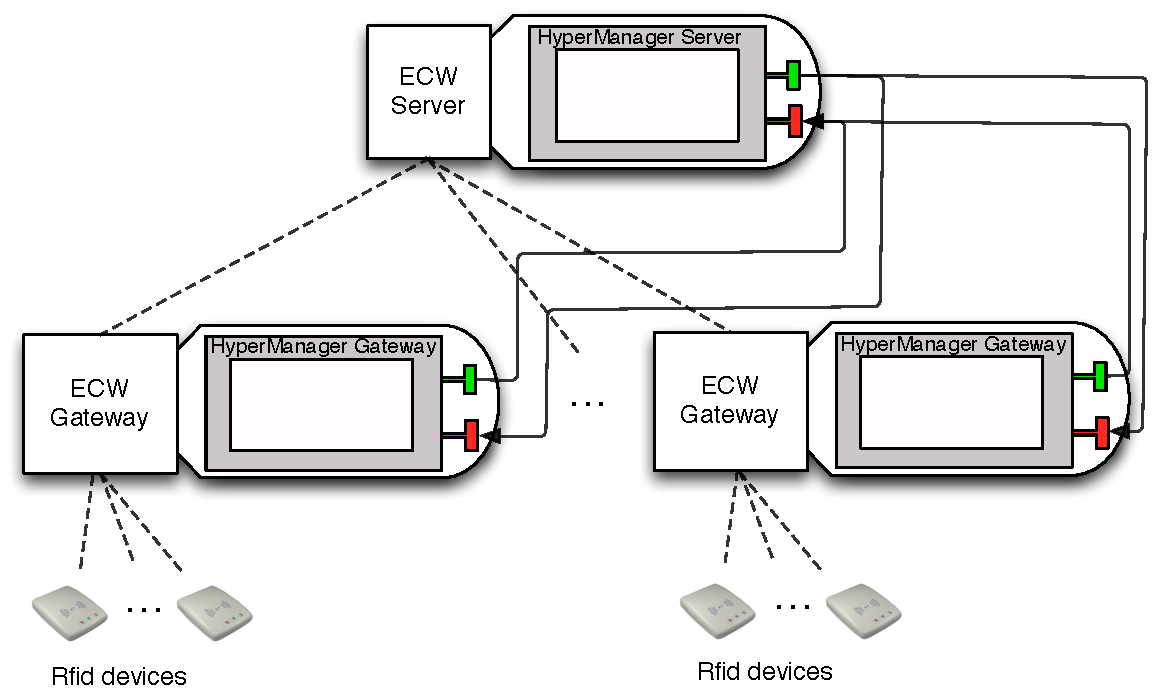
\includegraphics[scale=0.5]{figures/chapter3/architecture.pdf}
		\caption{Hierarchical representation of our case study}		
		\label{fig:hierarchy}
	\end{figure}

		
	Regarding the previously described scenario, this hierarchical view should pose no doubt.
	For each of the \textsc{n} floors of the hotel there are \textsc{m} laundry carts that interact in
	a \textit{one-to-one} style with a gateway.	On the other hand, the gateways communicate 
	with the server on a \textit{n-to-one} style. Moreover, there is also the need to cope for possible 
	maintenance issues. For instance, in the case of malfunction of some device running the \ac{ECW} \textsf{Gateway},
	it may be required to replace it or add a new one in order to avoid any overloading.
	 		 
	  				
	The architecture depicted by Figure \ref{fig:hierarchy}
	also includes \textsc{The HyperManager} application. Indeed, it is deployed alongside	the pre-existent
	distributed system, performing its monitoring on all \textsf{ECW} components. Moreover, the careful reader may notice 
	that the flow of requests go both from the \textsf{HyperManager Server} to
	the \textsf{HyperManager Gateway}, and vice-versa. Indeed, these follow the \textit{pull} and \textit{push}
	styles of communication, respectively. More details regarding these mechanisms will be discussed at a later stage.
	
		
	%%%
	\section[The HyperManager architecture]{The HyperManager architecture}
	\label{sub:thehm}
	
		 \textsc{The HyperManager} is a general purpose monitoring application that was developed 
	in the context of the Spinnaker project. The goal was to deliver a modular
	solution that would be capable of monitoring a distributed application and react to certain events.
	As such, \textsc{The HyperManager} is itself a distributed application, deployed alongside the target 
	application to monitor. %To simplify, we shall consider that this application is constituted by two levels.
	%The upper-level includes one server application, while the lower-level includes several gateways.
		
	Generally, when performing a monitoring task in an application one may consider two types of
	events: \textit{pull} and \textit{push}. The former stands for the usual communication scenario
	where the server regularly \textit{pulls} information from the client. The latter however, 
	is when the client \textit{pushes} data to the server. Both styles
	of communication are employed in \textsc{The HyperManager} application. %Figure \ref{fig:HMServer} depicts
	%the \textit{upper-level} of our \textsc{HyperManager}.
			
	\begin{figure}[H]
		\centering
		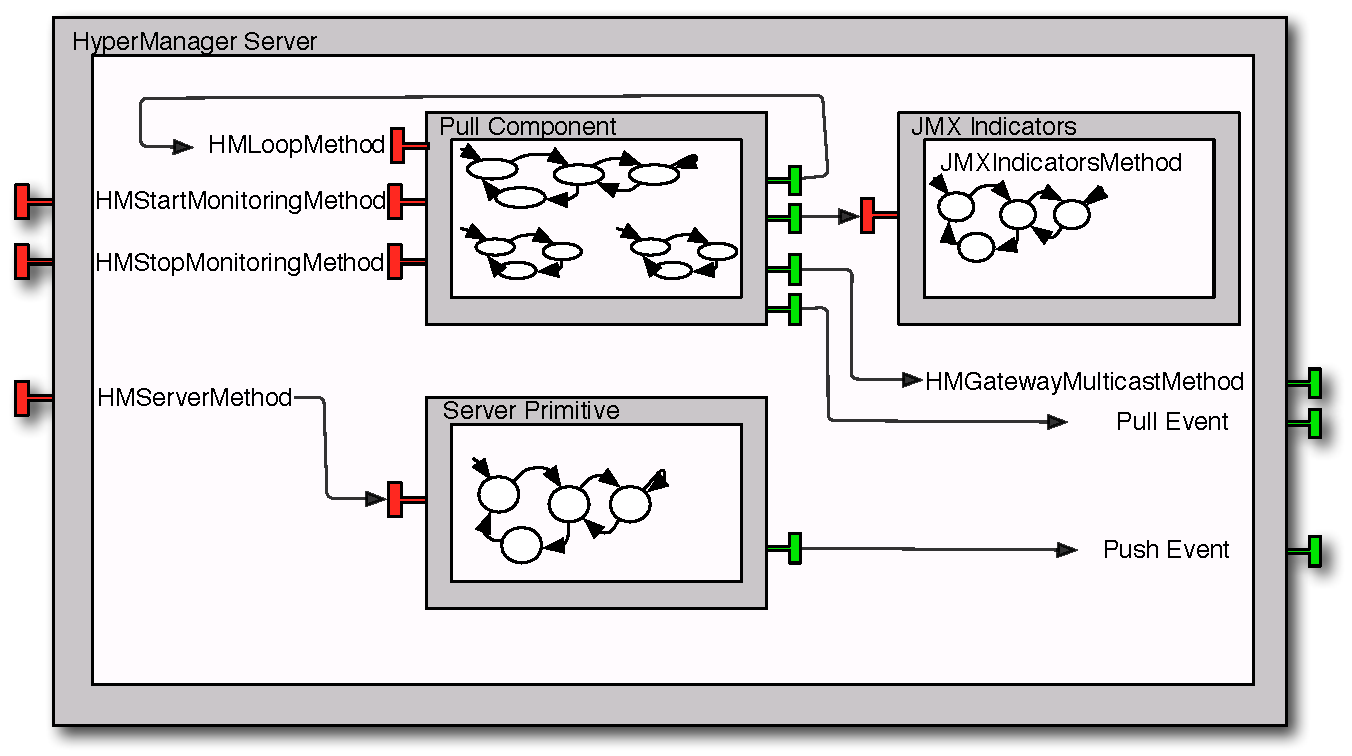
\includegraphics[scale=0.45]{figures/chapter3/HMServer-comp-v2.pdf}
		\caption{HyperManager server component}
		\label{fig:HMServer}		
	\end{figure}	
	
		
	As illustrated by Figure \ref{fig:HMServer}, the \textsf{HyperManager Server} component 
	features three primitive components that are responsible for	 the application logic. Each possesses  
	one or several service methods.
	
	The \textsf{JMX Indicators} component
	features only one service method: it accepts requests about a particular \ac{JMX}\footnote{\ac{JMX} is the standard protocol used for monitoring Java applications.}
	indicator and replies with its status. 
	This encapsulates business code and interacts directly with the \ac{ECW}.
	
	The \textsf{Pull Component} includes three service methods and four client interfaces. As the component's name indicates, it
	is responsible for \textit{pulling} information and emitting it as \textit{pull events}. The service methods \textsf{HMStartMonitoringMethod}
	and \textsf{HMStopMonitoringMethod} are responsible for starting and stopping the \textit{pulling} activity, respectively. Typically, these are the 
	methods called by an administrator. The remaining service method, \textsf{HMLoopMethod}, may pose some doubt. Indeed, it is called from
	one of its own client's interface. Being a \ac{GCM}/ProActive application, it follows the active object paradigm where explicit thread creation is discouraged.
 	As such, making a method \textit{loop} is achieved by making this method send itself a request before concluding its execution.	
 	
 	While in the monitoring loop, the \textsf{HMLoopMethod} method \textit{pulls} information regarding its own local \ac{JMX} indicators and those of its gateways 
 	via a multicast client interface. The last remaining client interface serves the purpose of reporting the \textit{pulled} information as \textit{pull} events.
		
	Last, the \textsf{Server Primitive} component receives \textit{push} information from the \textsf{HyperManager Gateway}s 
	--- typically to alert the occurrence of some anomaly --- and
	emits it as \textit{push} events. %In our implementation both \textit{push} and \textit{pull} events are then displayed
	%in some application with a graphical interface for administration purposes.
		
	The description of the \textsf{HyperManager Gateway} component follow the same spirit. Figure	 \ref{fig:HMGw} depicts its constitution.
	
	
	\begin{figure}[H]
		\centering
		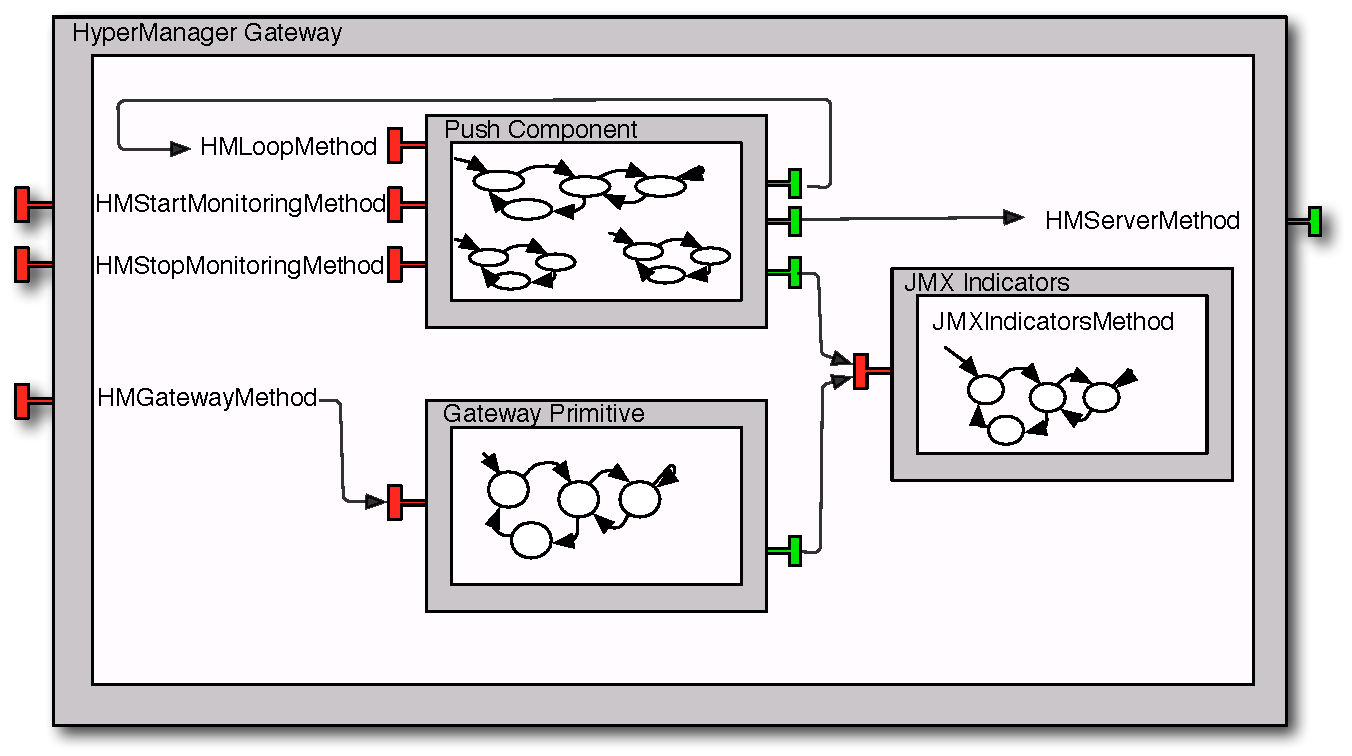
\includegraphics[scale=0.45]{figures/chapter3/HMGateway-comp-v2.pdf}
		\caption{HyperManager gateway component}
		\label{fig:HMGw}		
	\end{figure}		
	
	
	\noindent It is also composed of three primitive components. As expected, the \textsf{JMX Indicators} component has the same semantics as
	described above. 
	
	The \textsf{Push Component} features the same service methods as the \textsf{Pull Component}. Its semantics however, are slightly different.
	While \textit{looping} it will check for the status of its \ac{JMX} indicators, and communicate with  \textsc{The HyperManager} server if some anomaly
	is encountered --- which will then trigger a \textit{push} event.
	
	As for the \textsf{Gateway Primitive} component, its sole purpose is to reply to the \textit{pulling} requests from 
	the \textsf{HyperManager Server} component.
	

\section{Formal specification and verification methodology}		
\label{sec:methodology}		
		
		
			Regarding our modelling and verification \textit{workflow}, the first step is to build 
		the behavioural models by encoding the involved processes in the \textsf{Fiacre} specification 
		language. Naturally, this step can be partially automated as processes such as the \textsf{Queue},
		\textsf{Body}, etc, are computable, i.e., there is an algorithm that generates their behaviour. For instance,
		Listing \ref{lst:queuejmx} depicts the specification of the \textsf{Queue} process for the \textsf{JMX Indicators} 
		component in \textsf{Fiacre}. It should be noted that we need a finite representation of such process: 
		we illustrate this by a \textsf{Queue} bounded at two requests.
		
		
	\lstinputlisting[language=Fiacre,
	                        stepnumber=1, caption=Queue specification of the \textsf{JMX Indicators} component in Fiacre (bounded at two requests), 
	                        label=lst:queuejmx]{listings/chapter3/jmxqueue.tex}		

			
		%enqueuing is correct word	
	\noindent The \textsf{JMX Indicators} component possesses one service method, named
	\textsf{JMXIndicatorsMethod}, taking one argument of \textsf{JMXIndicatorsMethod\_args\_type}
	type. The three labels (lines 1-3) \textsf{Q\_JMXIndicatorsMethod}, \textsf{Serve\_JMXIndicatorsMethod} 
	and \textsf{Error} represent enqueuing of a request to its service method, 
	serving it, and throwing an exception due to exceeding of its capacity, 
	respectively. From \textsf{SEmpty}, upon reception of a request
	the process goes to state \textsf{S1} (lines 11-12), where it can serve the current request
	or receive another one (lines 14-17). The former case leads back 
	to \textsf{SEmpty}. The latter
	takes the execution to \textsf{S11} where it faces the same cases. 
	On the one hand, another request
	will lead to \textsf{SOutOfBounds} (line 21), at which point 
	the action \textsf{Error!errmsg} is emitted since 
	the request queue's maximum capacity is reached 
	--- where \textsf{errmsg} is a variable holding
	information about the antecedent state --- 
	and the execution is transferred to the sink state \textsf{SError} (lines 24-25). 
	On the other hand, since it exhibits a \ac{FIFO} policy, serving a request (line 20) 
	is performed on the initial call by emitting \textsf{Serve\_JMXIndicatorsMethod!a0,a00},
	and performing two assignments: \textsf{a0:=a1} and \textsf{a00:=a11}. The variables
	\textsf{a00}, \textsf{a11}, \textsf{a22} hold the request arguments by order of arrival. Thus, 
	this simple mechanism ensure they are served in an adequate order, i.e., 
	meeting the \ac{FIFO} policy. Moreover, the variables \textsf{a0}, \textsf{a1} and \textsf{a2}
	contain future proxies, and are handled analogously. Naturally, these are implicit --- transparent
	to the programmer ---, but included into the formal model.

		Let us now see how the \textsf{body} process is modelled. As an example, listing \ref{lst:bodyjmx} 
		depicts its specification for the \textsf{JMX Indicators} component.

			\lstinputlisting[language=Fiacre,
	                        stepnumber=1, caption=Body specification of the \textsf{JMX Indicators} component in Fiacre, 
	                        label=lst:bodyjmx]{listings/chapter3/jmxbody.tex}		
		
	
	\noindent Its understanding should pose no doubt. Basically, it idles in state \textsf{s0} until
	\textsf{Serve\_JMXIndicatorsMethod?fid,args} is activated, at which point the execution goes to \textsf{s1} (lines 10-11).
	From \textsf{s1} it emits \textsf{Call\_JMXIndicatorsMethod!fid,args}, therefore starting the actual method
	execution, and moves to \textsf{s11} (lines 13-14). Then, it just waits for the \textsf{JMXIndicatorsMethod} method 
	finish its execution and return, at which point \textsf{R\_JMXIndicatorsMethod?fid,reply} is received, and 
	it goes back to \textsf{s0} (lines 16-17).	
	
		\textsf{Proxy} and \textsf{ProxyManager} processes' behaviour can also be obtained in a systematic 
	manner. Together with the \textsf{Queue} and \textsf{Body} processes they model all the internal
	intricacies of a \ac{GCM} primitive component. The specification of the featured service methods however,
	is of specific nature, and thus a manual task.    
	
	
		Having the Fiacre sources files for all involved processes, we use the \textsc{flac} 
	compiler\footnote{Available online \url{http://gforge.enseeiht.fr/projects/fiacre-compil}} to 
	produce \textsc{Lotos} \cite{Bolognesi:1987:IIS:44211.44214}.
   Then,  we take advantage of the panoply of tools offered by the 
   CADP suite \cite{garavel:inria-00583776} for model generation and formal
   verification by model-checking techniques. Figure \ref{fig:workflow} depicts the overall 
   approach.
          		
	\begin{figure}[H]
		\centering
		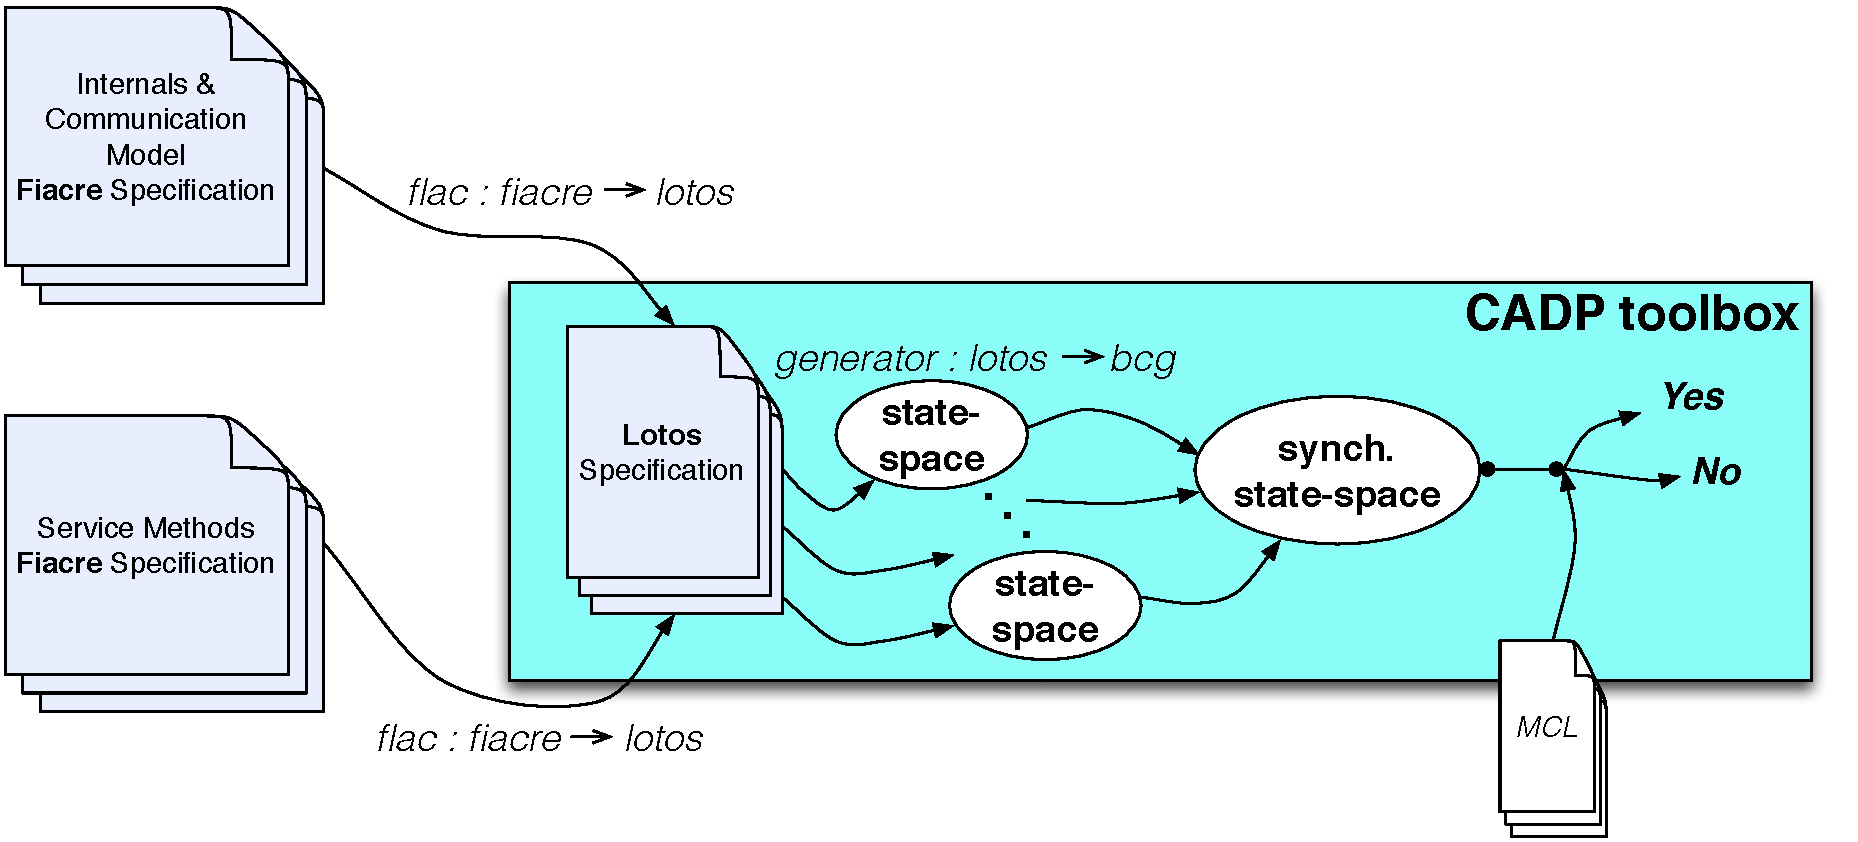
\includegraphics[scale=0.45]{figures/chapter3/mc.pdf}
		\caption{Formal specification and verification workflow}
		\label{fig:workflow}		
	\end{figure}		

	%%%pacagrid ... NEF..
	From CADP, we use \textsf{generator} for state-space generation. This process takes a plaintext
	\textsf{.lotos} file and yields a binary \textsf{.bcg} file encoding a \ac{LTS} that models
	the process behaviour. This file is usually referred to as the state-space. Moreover,
	it should be noted that state-space generation can be performed in a distributed manner.
	CADP's \textsf{distributor} tool implements a distributed algorithm that can be executed on several 
	machines. This can be of great value as	
	each of them is used to generate and store a part of the \ac{LTS}. 
	
		For the purposes of this thesis, we used distributed state-space generation by exploiting
	ProActive \textsf{PACA Grid} --- a computing cloud operated by INRIA, 
	University of Nice, and CNRS-I3S laboratory, and accessible through the 
	ProActive Scheduler\footnote{\url{http://proactive.activeeon.com/index.php?page=proactive_5_min}}.		
	Nevertheless, it should be noted that 	parallel composition through synchronization vectors
	is a sequential process, and thus may be a bottleneck for large systems. Indeed, as we shall see
	later, dealing with large state-spaces was one of the main challenges of this case study.
	
		
	%Typical file management and \ac{LTS} manipulation is conveniently achieved through \ac{SVL} scripts.
	%These encompass commands for state-space generation, label renaming and \ac{LTS} synchronization.
					
    %.exp which describes a network of communicating automata in the EXP 2.0 language defined below
    %svl - Script Verification Language	
				
			 For last, we use \textsf{evaluator4} for model-checking state-spaces against 
    \ac{MCL} \cite{Mateescu:2008:MCL:1423684.1423700} formulas --- an extension of the
    alternation-free regular $\mu$-calculus \cite{WinskellMuCalc} with facilities for manipulating data.		

		In the following, to optimize the size of the model, composite components have no request queue and 
	requests are directly forwarded to the
    targeted primitive component. This has no influence in the system's semantics as the request queues of the primitive components are sufficient for dealing with asynchrony and requests from the subcomponents are directly 
    dispatched too. We set the primitive components 
    with re-entrant calls --- \textsf{Pull Component} and \textsf{Push Component} --- with a \textsf{queue} 
    of size 2, and the remaining from the \textsf{HyperManager Server}  
    and \textsf{HyperManager Gateway} composites with size 1 and 2, respectively. Furthermore,
	we set the future proxy domain to range over \{0..1\}, and consider the existence of
    two \ac{RFID} devices per gateway.

\section{The HyperManager as a formal methods case study}
\label{sec:spec}

		
		As mentioned above, \textsc{The HyperManager} is a \ac{GCM}/ProActive application. A natural
	choice for its behavioural specification is therefore pNets. This task requires the specification
	of all service methods composing the application. These transparently interact with
	the component's internal intricacies --- component queue, proxy manager, ... ---, 
	that are also included in the model.
	
		In the following we dedicate Subsection \ref{sub:hmgwverif},
		Subsection \ref{sub:hmserververif}, and Subsection \ref{sub:prod1} to the discussion
		on the specification and verification by model-checking of the \textsf{HyperManager Gateway} component,
		\textsf{HyperManager Server} component, and overall system product, respectively.
		Next, Section \ref{sec:reconfig} deals with the inclusion of structural reconfigurations
		in our model. Section \ref{sec:hyperremarks} gives some final
		remarks regarding this case study.
	
		Moreover, for more material on this case study --- namely the specification's source files ---,
		the reader is invited to check its companion 
		website\footnote{\url{http://www-sop.inria.fr/members/Nuno.Gaspar/HyperManager.php}}.	
	
	  

    

\subsection{On HyperManager Gateway}
\label{sub:hmgwverif}


\subsubsection{\textsf{JMX Indicators} component}	

	As seen above, the \textsf{JMX Indicators} primitive component only features one service method, 
	\textsf{JMXIndicatorsMethod}, with \textsf{JMXIndicatorsMethod\_args\_type} and 
	\textsf{JMXIndicatorsMethod\_return\_type} as argument and return types, respectively. These
	are specified as shown by Listing \ref{lst:typesjmx}.

			\lstinputlisting[language=Fiacretypes,
	                        stepnumber=1, caption=Specification for the \textsf{JMXIndicatorsMethod} argument and return types, 
	                        label=lst:typesjmx]{listings/chapter3/jmxtypes.tex}	


	\noindent For the sake of simplicity, we only model two 
	types of \ac{JMX} indicators: \textsf{MemoryUsage} and \textsf{DeviceStatus}. The latter takes into account an identifier, 
	returning its availability status. This relates to the status of a \ac{RFID} reader transmitting to the \ac{ECW} Gateway.
	While the former accounts for the stability status of the memory. 
	
	%JMX no servidor nao tem isso... contextual stuff: synch. with a context that only sends memory status requests
	%compositional

	Listing \ref{lst:mjmx} illustrates the specification of the \textsf{JMXIndicatorsMethod} method behaviour.
	
		\lstinputlisting[language=Fiacre,
	                        stepnumber=1, caption=\textsf{JMXIndicatorsMethod} specification, 
	                        label=lst:mjmx]{listings/chapter3/jmxm.tex}		
	
	
	\noindent Basically, it waits at the \textsf{s\_init} state until it receives a request call regarding
	one of the \ac{JMX} indicators (lines 11-13). Then, it goes to state \textsf{s\_mem} or
	\textsf{s\_dev}, depending on which \ac{JMX} indicator is queried:
	a request to the memory usage takes the execution
	to the former, while a request to the device statuses takes the execution to the latter.
	From \textsf{s\_mem} it randomly replies one of the possible values for
	the memory usage and goes back to \textsf{s\_init} (lines 16-19). As expected, the 
	same behaviour w.r.t. device statuses occurs from \textsf{s\_dev} (lines 21-22).
	The careful reader may wonder about	the rather different specification approaches
	between the reply of the two \ac{JMX} indicators. Indeed, for the memory usage it 
	exhaustively lists all possible reply values, and emits a non-deterministic choice among them.
	For the devices statuses however, it simply replies with a non-instantiated variable \textbf{x},
	that does the work of ranging over all possible reply values. Naturally, both approaches have 
	the same semantics, it is merely a matter of style.
	
	
	The Fiacre specification language allows for fairly simple and intuitive descriptions of 
	automata-based models. Nevertheless, a more convenient representation for 
	illustrating automata is in its graphical form. For instance, Figure \ref{fig:JMX} depicts 	
	the behaviour of the \textsf{JMXIndicatorsMethod} method.	
	
	\begin{figure}[H]
		 \centering
		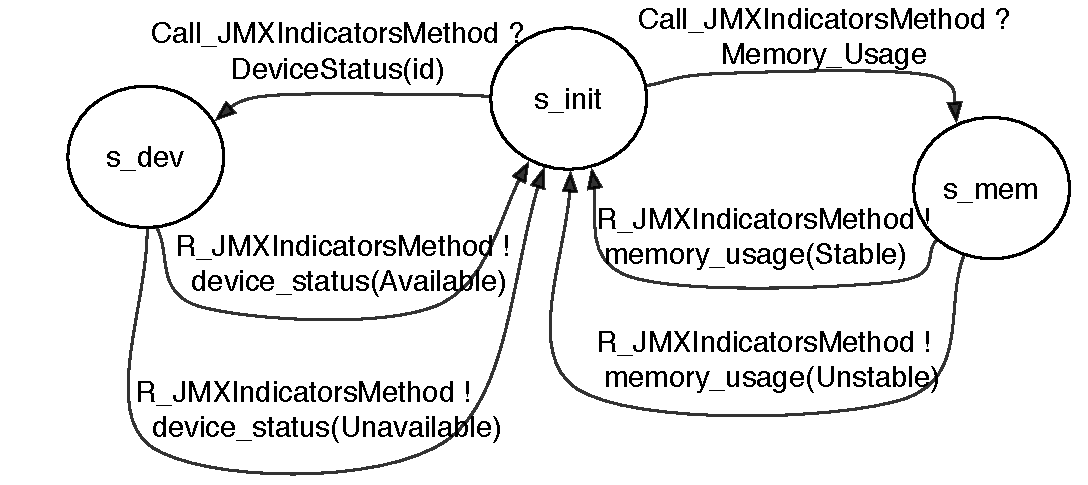
\includegraphics[scale=0.6]{figures/chapter3/JMXIndicatorsMethod.pdf}
		\caption{Behaviour of the JMXIndicatorsMethod method}
		\label{fig:JMX}		
	\end{figure}			
	
		
	\noindent Its understanding is straightforward, as it closely follows Fiacre's specification
	from Listing \ref{lst:mjmx}. There is, however, one	 small nuance: it does not include the 
	future proxies. Indeed, these are related to the internal machinery of 
	\ac{GCM} components, and one would rather avoid such intricacies when specifying service
	methods. As such, they are omitted in the graphical representations: we consider these representations
	as an \textit{user-version} \ac{LTS}, i.e., typically what a user would specify without paying 
	attention to the future proxies mechanism. 
			

\subsubsection{\textsf{Gateway Primitive} component}	
	
	Let us now look at the behaviour of the \textsf{HMGatewayMethod} method. Listing
	\ref{lst:mgw} details its specification in Fiacre.		
	
	\lstinputlisting[language=Fiacre,
	                        stepnumber=1, caption=\textsf{HMGatewayMethod} specification, 
	                        label=lst:mgw]{listings/chapter3/gwm.tex}		
			
	\noindent Despite its apparatus, this service method offered by the \textsf{Gateway Primitive} component 
	has also a fairly simple semantics. It acts merely as a request forwarder for the \textsf{JMX Indicators} component.
	A far more convenient specification is given by Figure \ref{fig:GwM}.	
	     
	\begin{figure}[H]
		 \centering
		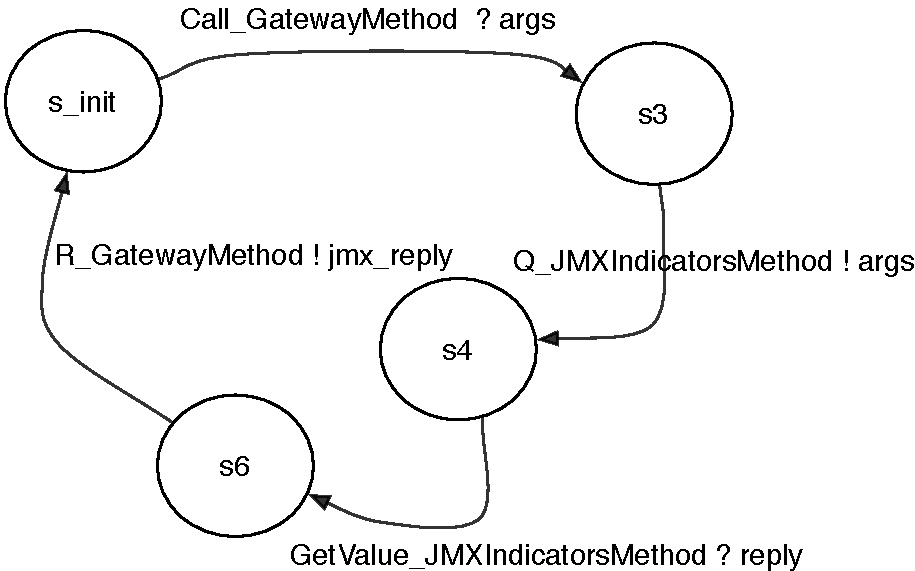
\includegraphics[scale=0.6]{figures/chapter3/HMGatewayMethod.pdf}
		\caption{Behaviour of the HMGatewayMethod method}
		\label{fig:GwM}		
	\end{figure}		

	
	\noindent For this example the extra verbosity introduced by the handling of future proxies is even
	more evident. Indeed, all this machinery ends up obfuscating the method's actual behaviour.		
	In the following, we constrain ourselves to the \textit{user-version} \ac{LTS} representation for 
	the description of service method behaviour. Hopefully, this shall facilitate the understanding
	of the remaining specifications.		


\subsubsection{\textsf{Push Component} component}	
	
	
	Regarding the \textsf{Push Component}, it is composed by three service methods:  \textsf{HMStartMonitoringMethod},
	\textsf{HMStopMonitoringMethod} and \textsf{HMLoopMethod}. Further, the global variable \textbf{started} is shared
	among them. For the sake of clarity communication actions are 
	written in black, while \textit{local} computations (e.g. guard evaluations, assignments) are written in blue. 
	Their intended meaning should pose no doubt.
	
	   \begin{figure}%[H]
	\centering
	\begin{minipage}[b]{0.45\linewidth} 
	\centering
	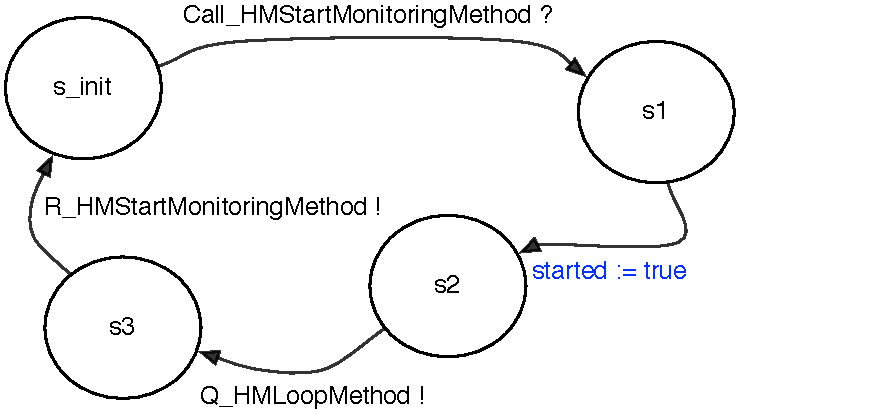
\includegraphics[width=\textwidth]{figures/chapter3/HMStartMethod.pdf}
	\caption{Behaviour of the HMStartMonitoringMethod method}
	\label{fig:start}
	\end{minipage}
	\hspace{0.10cm}
	\begin{minipage}[b]{0.45\linewidth} 
	\centering
	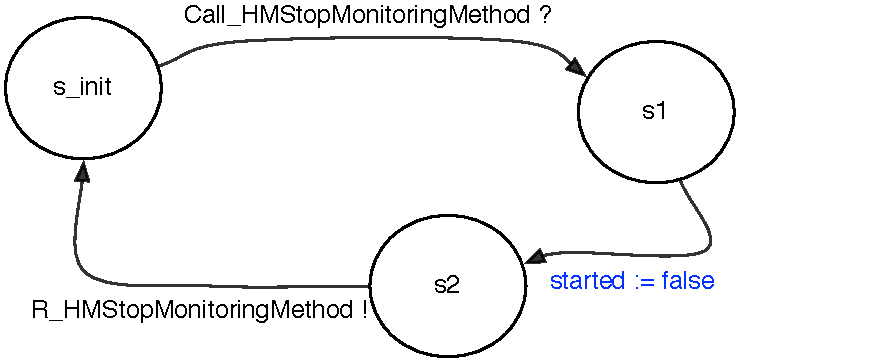
\includegraphics[width=\textwidth]{figures/chapter3/HMStopMethod.pdf}
	\caption{Behaviour of the HMStopMonitoringMethod method}
	\label{fig:stop}
	\end{minipage}
	\end{figure}	  
		
	Figure \ref{fig:start} and Figure \ref{fig:stop} depict the behaviours of the \textsf{HMStartMonitoringMethod} and 
	\textsf{HMStopMonitoringMethod} methods, respectively. Basically, they are responsible for	
	enabling/disabling the \textit{looping} process of the \textsf{HMLoopMethod}. This is achieved 
	by the shared variable \textbf{started}. On the one hand, invoking \textsf{HMStartMonitoringMethod} sets \textbf{started} 
	to \textit{true} and performs an invocation to \textsf{HMLoopMethod}. On the other hand, 
    \textsf{HMStopMonitoringMethod} sets \textbf{started} to \textit{false}. 

	It should be noted that these local computations involving the global variable \textbf{started} are
	merely syntactic sugar for the emission and reception of messages to another process. In practice, 
	the involved labels  are \textsf{GuardQuery}, \textsf{GuardReply?b:bool}, \textsf{SetFalse} and \textsf{SetTrue}.
	Their meaning should be obvious from their labels.
		
	The last remaining service method	to describe is the most interesting one --- the \textsf{HMLoopMethod} 
	method. Its behaviour is depicted by Figure  \ref{fig:LG}. 
	
\begin{figure}%[H]
	\centering
		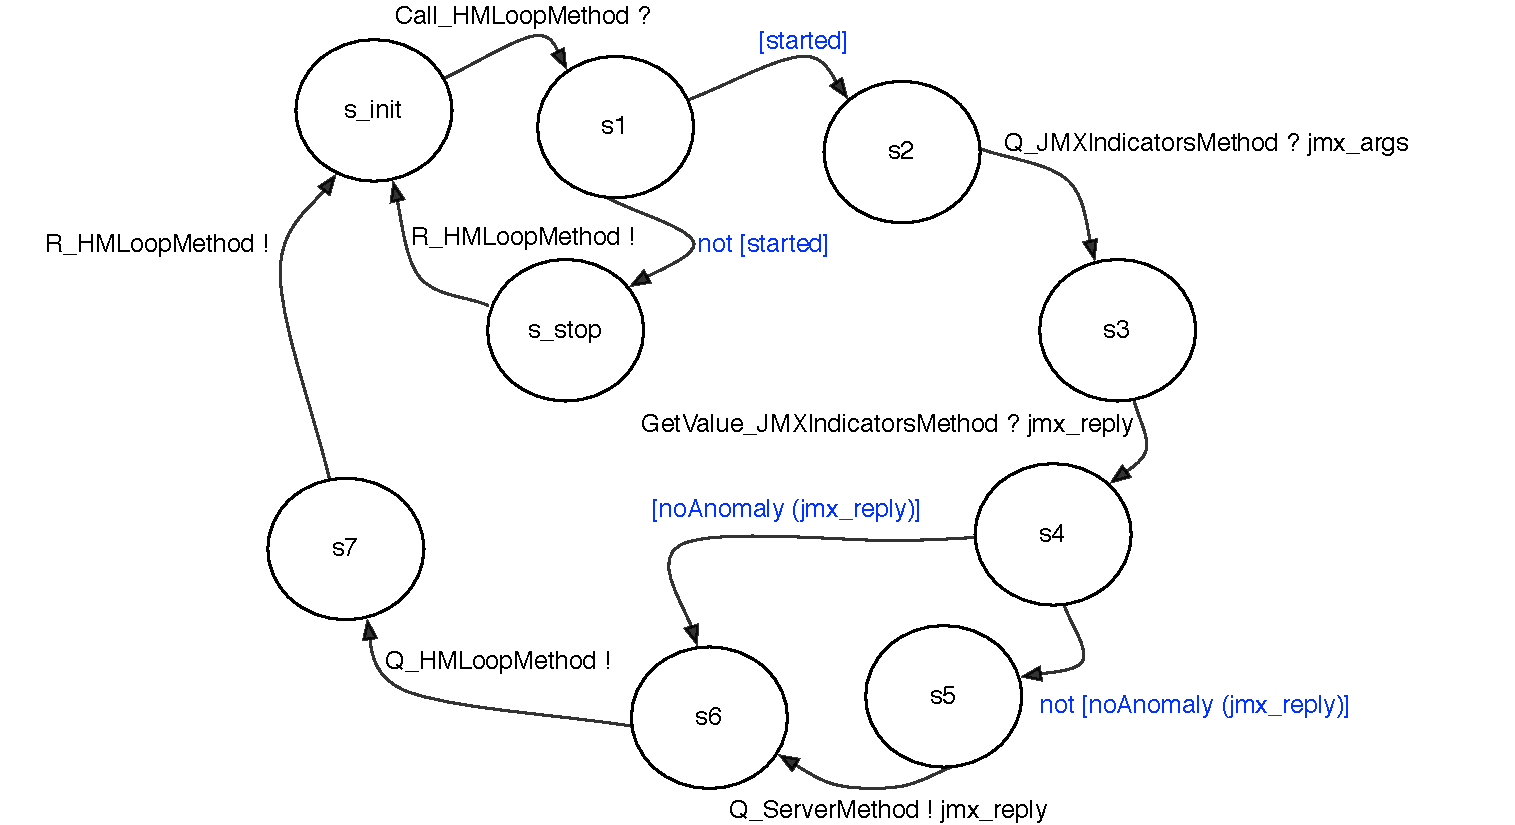
\includegraphics[scale=0.5]{figures/chapter3/HMLoopMethodatGateway.pdf}
		\caption{Behaviour of the HMLoopMethod method for the HyperManager Gateway}
		\label{fig:LG}		
\end{figure}	
	
	\noindent The reception of \textsf{Call\_HMLoopMethod} action starts the method execution, 
    moving from state \textsf{s\_init} to state \textsf{s1}. Then, the global variable \textbf{started} is checked.
    If it evaluates to \textit{false} the method returns by emitting a \textsf{R\_HMLoopMethod}
    message. Otherwise, the execution proceeds by querying the gateway's local \ac{JMX} indicators 
    --- from \textsf{s2} to \textsf{s3} through \textsf{Q\_JMXIndicatorsMethod?jmx\_args}. The reply
    is received by \textsf{GetValue\_JMXIndicatorsMethod?jmx\_reply} and evaluated at state \textsf{s4}.
	If an anomaly is detected (e.g. unstable memory), it is reported to the \textsf{HyperManager Server} component
	through the message \textsf{Q\_ServerMethod!jmx\_reply}, thus 
	moving from state \textsf{s5} to state \textsf{s6}. If no anomaly is found, the execution proceeds directly
	to state \textsf{s6}, where a call to the method itself is performed: \textsf{Q\_HMLoopMethod}. This places
	a request on the \textsf{Push Component} component queue --- thus making the method \textit{loop} --- and
	transfers the execution to state \textsf{s7}. It should be noted that this request is scheduled as any other 
	one: the \ac{FIFO} policy dictates that requests are served by order of arrival, and therefore a potential
	 \textsf{Q\_HMStopMonitoringMethod} enqueued in the meantime would be served before this new 
	 \textsf{Q\_HMLoopMethod} request.        
	Finally, from state \textsf{s7}, the message \textsf{R\_HMLoopMethod} is emitted, and the method execution
	concludes by going back to state \textsf{s\_init}.
  


\subsubsection{Model Generation and Proven Properties}
		
		Model generation is performed by synchronizing all the involved processes --- 
		\ac{GCM} internals and service methods --- of the \textsf{HyperManager Gateway} component.		
		Table \ref{tab:modelG} illustrates its state-space information. 		

\begin{table}[H]
\begin{center}
\begin{tabular}{| l | c | c | c | c |}
\hline
                             &  \textbf{States} & \textbf{Transitions} & \textbf{File Size} \\
\hline
   \textsf{hmgateway.bcg}            &  14.931.628  &  147.485.103  &  $\sim$ 295 mb\\
  \hline
\end{tabular}
\end{center}
\caption{State-space information for the \textsf{HyperManager Gateway} component}
\label{tab:modelG}
\end{table}

	  
	Having the state-space generated we can now prove some properties regarding the expected behaviour of the model.
	Specifying properties of interest in \ac{MCL} is a rather intuitive task due to its expressiveness and conciseness. 
	Its main ingredients include patterns extracting data values from \ac{LTS} actions,
	modalities on transition sequences described using extended regular expressions, 
	and programming language constructs.
	
	For instance, one could  wonder about this rather unusual \textit{looping} mechanism. Once 
	setting the global variable \textsf{started} to \textit{true} 
	--- accomplished by \textsf{Q\_HMStartMonitoringMethod} ---, the \textit{looping} continues until a 
	request to stop monitoring is received. That is, there is no execution path in 
	which the global variable \textbf{started} evaluates to \textit{false} without the occurrence of 
	a \textsf{Q\_HMStopMonitoringMethod}.	 Property \ref{prop:loopsgw} encodes this statement in \ac{MCL}.


%loop-while-flag-true
\begin{property}[loops while variable started is true]
\label{prop:loopsgw}
\begin{verbatim}
	
	[ "Q_HMStartMonitoringMethod" . 
	     (not "Q_HMStopMonitoringMethod")* . "GuardReply !FALSE" ] false
\end{verbatim}
\end{property}%2m48s


	\noindent More precisely, Property \ref{prop:loopsgw} reads: all paths starting with the label \textsf{Q\_HMStartMonitoringMethod},
	followed by any other sequence of labels not including \textsf{Q\_HMStopMonitoringMethod}, and
	ending by \textsf{GuardReply !FALSE}, cannot occur. Model-checking \textsf{hmgateway.bcg}  against this formula
	demonstrates that it is indeed true.
	

	Another property of interest concerns the overloading of the \textsf{HyperManager Server} component
	with unnecessary messages. We want to ensure that we cannot
	\textit{push} data if not in the presence of an anomaly. This is modelled by Property \ref{prop:overload}.

\begin{property}[no server overload]
\label{prop:overload}

 \begin{verbatim}
 
[ ((not "R_JMXIndicatorsMethod !memory_usage (Unstable)")* . 
       "Q_ServerMethod.*")  |
  ((not "R_JMXIndicatorsMethod !device_status ((Unavailable, IdTwo))")* . 
       "Q_ServerMethod.*") |
  ((not "R_JMXIndicatorsMethod !device_status ((Unavailable, IdOne))")* . 
       "Q_ServerMethod.*") 
] false
 \end{verbatim}
  \end{property}


	\noindent The above \ac{MCL} formula states that all paths starting with any sequence of labels
	not including the reply of an anomalous \ac{JMX} indicator --- \textsf{R\_JMXIndicatorsMethod !memory\_usage (Unstable)},
	\textsf{R\_JMXIndicatorsMethod !device\_status ((Unavailable, IdTwo))} and 
	\textsf{R\_JMXIndicatorsMethod !device\_status ((Unavailable, IdOne)} ---, followed by
	a \textsf{Q\_ServerMethod.*} --- where * is a \textit{wildcard} matching all possible arguments ---, cannot occur.	
	With no surprise, Property \ref{prop:overload} is also proved to be satisfied by the model.


\subsection{On HyperManager Server}
\label{sub:hmserververif}
	
	
\subsubsection{\textsf{JMX Indicators} component}		
	
		As seen for the \textsf{HyperManager Gateway} component, the \textsf{HyperManager Server} component also features 
	a 	\textsf{JMX Indicators} component.	This one however, is not endowed with \ac{JMX} indicators
	for the \ac{RFID} devices statuses. 
	
		Technically, we attach to the \ac{LTS} modelling the behaviour of the \textsf{JMX Indicators}
		component (see Figure \ref{fig:JMX})
	a context that constraints its requests. This is achieved by synchronization with another \ac{LTS}
	that solely emits requests regarding the memory status. This approach for contextual state-space 
	generation is compositional and thus promotes reusability. 
		

\subsubsection{\textsf{Server Primitive} component}		

   As seen above, upon detection of an anomaly, the \textsf{HyperManager Gateway} components \textit{push} 
   the relevant information to the \textsf{HyperManager Server}. Then, it is emitted as a
  \textit{push} event. This behaviour is depicted by Figure \ref{fig:SM}. 
  
	\begin{figure}[H]
		\centering
		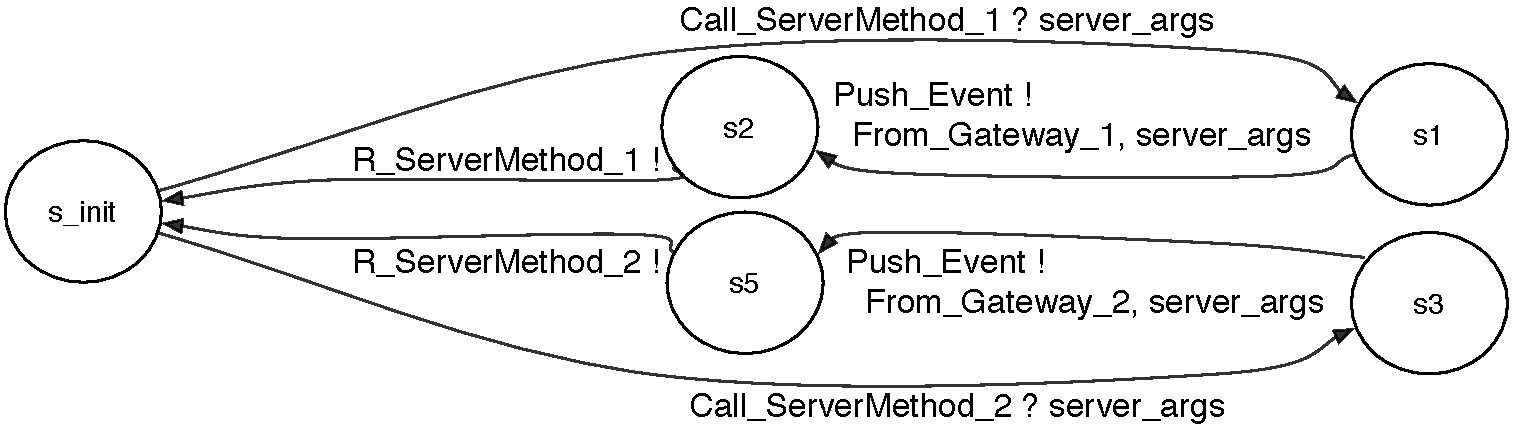
\includegraphics[scale=0.5]{figures/chapter3/HMServerMethod.pdf}
		\caption{Behaviour of the HMServerMethod method}
		\label{fig:SM}		
	\end{figure}	  
  
  \noindent The careful reader will notice that the emitted event also contains
   the information regarding the \textsf{HyperManager Gateway} component from which 
   the anomaly originated. This should come as no surprise as there can be
   several of them, and properly identifying the source of an abnormal situation 
   is of paramount importance. In our model, we consider the existence of two 
   \ac{ECW}/HyperManager gateways, and therefore we include specific labels
   --- \textsf{Call\_ServerMethod\_i}$_{i\in\{1,2\}}$ and  \textsf{R\_ServerMethod\_i}$_{i\in\{1,2\}}$ --- 
	for  communicating with them.
  
  
\subsubsection{\textsf{Pull Component} component}		  
  		
	
	The \textsf{Pull Component} component is composed by three service methods: \textsf{HMStartMonitoringMethod},
	\textsf{HMStopMonitoringMethod}, and \textsf{HMLoopMethod}. Indeed, these have the same names as the service methods
	for the \textsf{Push Component} component. In fact, their \textsf{HMStartMonitoringMethod} and 
	\textsf{HMStopMonitoringMethod} methods possess the same semantics (depicted by Figure \ref{fig:start} 
	and Figure \ref{fig:stop}). Their \textsf{HMLoopMethod} method however, behave differently.
    Figure \ref{fig:LS} depicts its behaviour for the \textsf{Pull Component}.

	\begin{figure}[H]
	\centering
		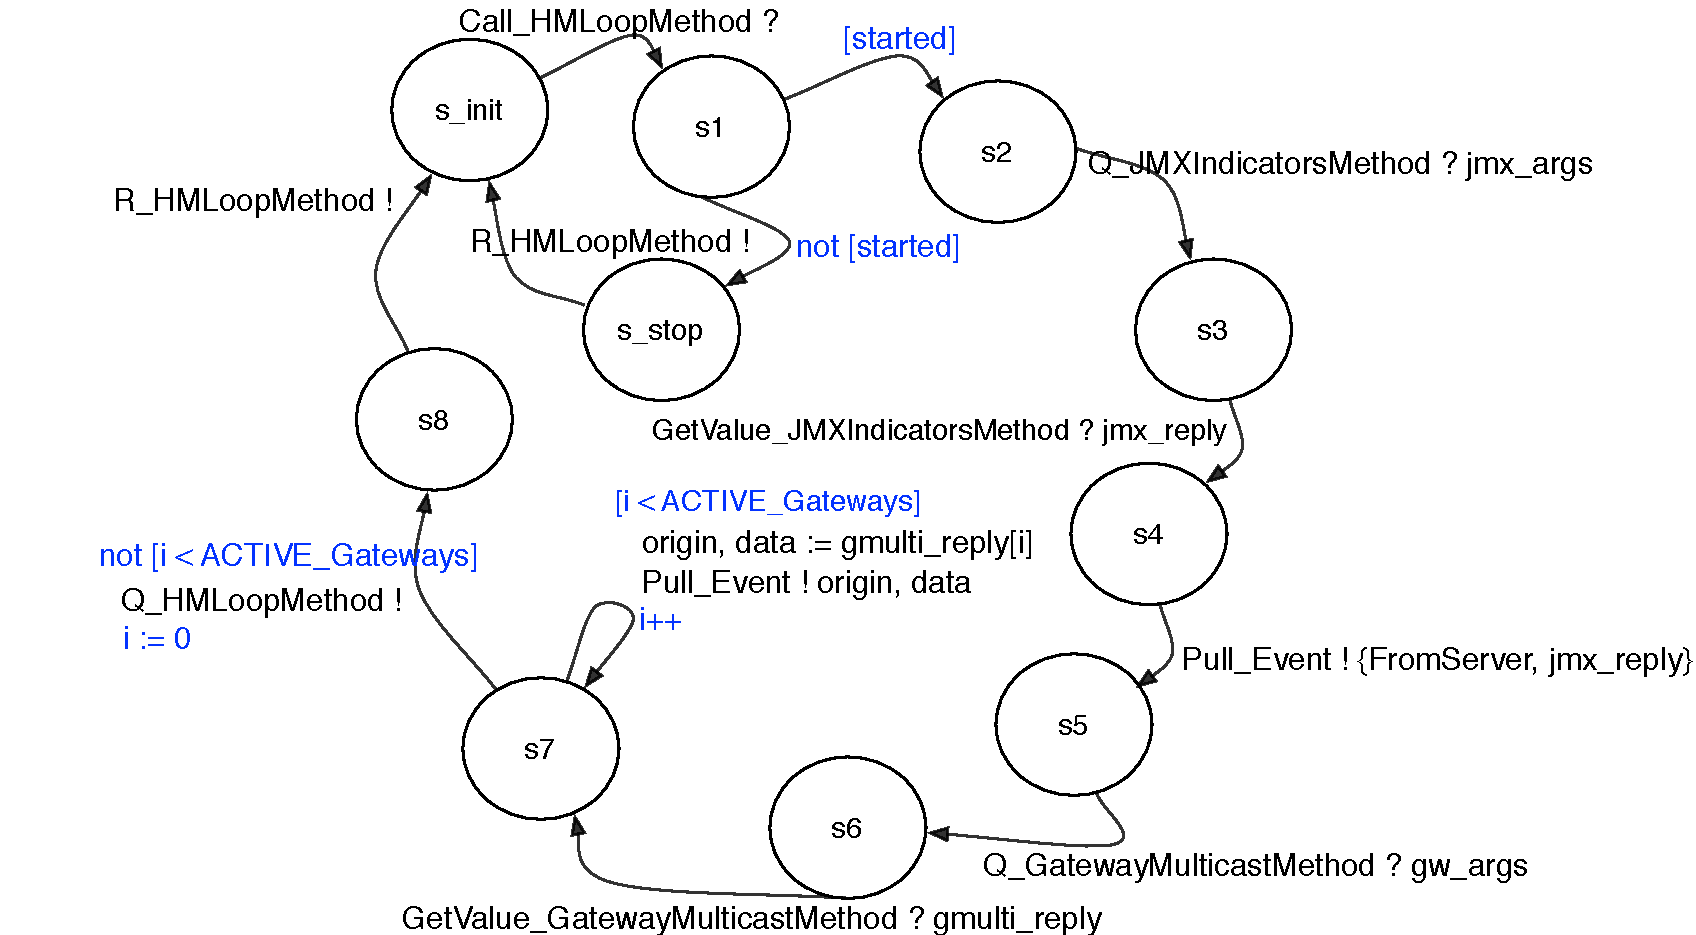
\includegraphics[scale=0.5]{figures/chapter3/HMLoopMethodatServer2.pdf}
		\caption{Behaviour of the HMLoopMethod method for the HyperManager Server}
		\label{fig:LS}		
	\end{figure}	  

	\noindent Its \textit{looping} mechanism is also handled through a shared 
	variable named \textbf{started}.  While \textit{looping}, 
	the local \ac{JMX} indicators are queried, and its reply emitted 
	as \textit{pull} events. Moreover, through the multicast interface 
	the monitoring information is \textit{pulled} from the bound gateways. 
	This, emits as many \textit{pull}
    events as the number of bound gateways. Last, a request to 
    itself is performed in order to continue \textit{looping}.


\subsubsection{Model Generation and Proven Properties}


	Table \ref{tab:modelS} illustrates the relevant information concerning \textsf{HyperManager Server}'s 
	state-space.

\begin{table}[H]
\begin{center}
\begin{tabular}{| l | c | c | c | c |}
\hline
                             &  \textbf{States} & \textbf{Transitions} & \textbf{File Size} \\
\hline
  \textsf{hmserver.bcg}                                   &   12.787.376   &  187.589.422  &  $\sim$  363 mb\\
  %\textsf{hmserver-min.bcg}    &   12.787.376  &   187.589.422 &   $\sim$  396 mb \\
  \hline
\end{tabular}
\end{center}
\caption{State-space information for the \textsf{HyperManager Server} component}
\label{tab:modelS}
\end{table}

		
	It should be noted that we can also prove properties regarding the \ac{GCM} internals.
	For instance, a rather trivial property we can expect to hold is that we can reach a state 
	which exceeds the maximum capacity of the request queue. 
	For the \textsf{Server Primitive} component, this can be modelled in \textsf{MCL} as demonstrated
	by Property \ref{prop:queueex}
  	
	\begin{property}[reachable exception]
	\label{prop:queueex}
	\begin{verbatim}
	
		< true* . 'QueueException_ServerPrimitive !.*'> true
	\end{verbatim}
	\end{property}

	\noindent Formally, this property reads: from any state, there exists an execution path that can encompass the label
	\textsf{QueueException\_ServerPrimitive !.*}. As expected, this property is proved to be satisfied by the model.
	
		Another property regarding the \ac{GCM} internals concerns the use of proxies. For instance,
	the \textsf{HMLoopMethod} needs to request
	a proxy in order to be able to invoke the service method from the \textsf{JMX Indicators} component. 
	This is encoded as demonstrated by Property \ref{prop:proxy}.
	
	 \begin{property}[need for proxy]
	\label{prop:proxy}	 
	 
	\begin{verbatim}
	
		[ (not "GetProxy_JMXIndicatorsMethod.*")* . 
		             "Q_JMXIndicatorsMethod.*"] false
	\end{verbatim}
   \end{property}
	%proved true. job #3128 (proxy_request2.mcl)
	%2h 24m
   
   \noindent Formally, the above property reads: all execution paths starting with any sequence of labels not including
   \textsf{GetProxy\_JMXIndicatorsMethod.*}, and followed by \textsf{Q\_JMXIndicatorsMethod.*}, cannot occur.
    With no surprise, model-checking this property confirms that it is satisfied by the model.
	    
\subsection{On System Product}
\label{sub:prod1}

	%- space state explosion phenomena
   %- action communication hiding
 
 	%We generated the product of our system	with 2 gateways. Table \ref{tab:modelSP} shows the relevant information.
 	
	We attempted to generate a system product constituted by two \textsf{HyperManager Gateway}s and 
	one \textsf{HyperManager Server} components. However, even on a machine with 90 GB of RAM, we experienced
	the so common state-space explosion phenomena. Indeed, as discussed in Section \ref{sec:methodology},
	while we can use distributed state-space generation, and thus spread the workload among several machines,
	synchronizations products remain a sequential task. 
	
	This arises often in the analysis of complex systems. To this end, \textit{communication hiding} 	
	comes as an efficient and pragmatic approach for tackling this issue. Indeed, it allows the specification of 
	actions that need not to be observed for verification purposes, thus yielding
	more tractable state-spaces.
	
	Table \ref{tab:modelSP} illustrates the effects of applying this technique to the model. The sole
	\textit{communication actions} being hidden are the ones involved in (1) the request transmission
	from the \textsf{Queue} to the adequate method --- \textsf{Serve\_} and \textsf{Call\_} ---, 
	(2) the proxy machinery ---\textsf{GetProxy\_}, \textsf{New\_} and \textsf{Recycle\_} ---, 
	and (3) finally in the \textit{guard} of the \textit{looping} methods --- \textsf{GuardQuery},
	\textsf{GuardReply}, \textsf{SetFalse} and \textsf{SetTrue}. 
	

\begin{table}[H]
\begin{center}
\begin{tabular}{| l | c | c | c |}
\hline
                             &  \textbf{States} & \textbf{Transitions} & \textbf{File Size} \\
\hline
   \textsf{hmgateway-hidden.bcg}           & 14.931.628  & 147.485.103  &  $\sim$  287 mb\\
   \textsf{hmgateway-hidden-min.bcg}   &   409.374      & 4.007.232     &  $\sim$  8.5 mb\\
  \hline
   \textsf{hmserver-hidden.bcg}           &  12.787.376    & 187.589.422    &   $\sim$  375 mb\\
  \textsf{hmserver-hidden-min.bcg}   &      5.761.504 &  85.157.420   &   $\sim$  179 mb \\
  \hline
  \textsf{SystemProduct.bcg}                                &  342.047.684  & 3.026.114.393 &  $\sim$  5.27 gb\\
  \textsf{SystemProduct-min.bcg}   &  259.340.044  &  2.396.896.830  &  $\sim$  4.83 gb\\
 \hline
\end{tabular}
\end{center}
\caption{State-space information for the overall system product}
\label{tab:modelSP}
\end{table}

		The lines suffixed by \textsf{-hidden} indicate the results obtained by \textit{hiding}
		the mentioned \textit{communication actions} in the \textsf{HyperManager Gateway}
		and \textsf{HyperManager server} state-spaces. For both, no effect is noticed on the 
		size of the \ac{LTS}. However,
		there is a decrease in the file size. This is due to the fact that the \textit{hiding} process
		yields several $\tau$-transitions, which facilitates file compression. More importantly, this 
		has the consequence of leveraging the subsequent \textit{minimization} process:
		the entries suffixed by \textsf{-min} mean that minimization by branching \textit{bisimulation} 
		was applied.	 Indeed, we even obtain a reduction by two orders of magnitude (!) for the 
		\textsf{HyperManager Gateway} state-space. 
		
			%With
		
		\textsc{The HyperManager} comes as a monitoring application that should be able to properly
		trace the origin of an anomaly. As such, one behavioural property that we expect to hold is that
		whenever an abnormal situation is detected by a \textsf{HyperManager Gateway}, it is \textit{fairly inevitable} 
		to be reported as a \textit{push event} that correctly identifies its origin. 
		
		First, we shall use \ac{MCL}'s macro capabilities to help us build the formula:
		
		%\scalebox{0.5}{

		\begin{verbatim}
			macro GETVALUE_1_MEMORY () = 
			  "GetValue_JMXIndicatorsMethod_Push_1 !memory_usage (Unstable)" 
end_macro

macro PUSH_1_MEMORY ()     = 
  ("Push_Event (FirstGateway, UnstableMemoryUsage)")  
end_macro
...
		\end{verbatim} 

		
		\noindent The above macros should be self-explanatory. The former represents the detection of an anomaly
		coming from the first \textsf{HyperManager Gateway} --- the model is instantiated with two \textsf{HyperManager Gateway}s,
		thus we differentiate  their actions by suffixing them adequately. The latter stands for the emission
		of the \textit{push} event corresponding to that anomaly. The macros for the remaining
		relevant actions are defined analogously.
		
			Moreover, we define the following macro generically encoding the 
			\textit{fair inevitability}\footnote{We consider the definition by 
			Queille and Sifakis \cite{journals/acta/QueilleS83}: a sequence is fair iff it does not infinitely often 
			enable the reachability of a certain state without infinitely often reaching it.} that
			after an \textit{anomaly} the system emits a \textit{push}.
			
		\begin{verbatim}
			macro FAIRLY_INEVITABLY_A_PUSH (ANOMALY, PUSH) =
       [ true* . "ANOMALY" . (not "PUSH")* ]
           < (not PUSH)* . PUSH > true
end_macro
		\end{verbatim}		
		
		
		\noindent Having the macros defined, we can now write the formula of interest:


		\begin{property}[push fairly inevitable] 
		\label{prop:fair1}
			\begin{verbatim}	
			
(FAIRLY_INEVITABLY_A_PUSH(GETVALUE_1_MEMORY, PUSH_1_MEMORY) and
 FAIRLY_INEVITABLY_A_PUSH(GETVALUE_2_MEMORY, PUSH_2_MEMORY) and
 FAIRLY_INEVITABLY_A_PUSH(GETVALUE_1_DEVICE_1, PUSH_1_DEVICE_1) and
 FAIRLY_INEVITABLY_A_PUSH(GETVALUE_1_DEVICE_2, PUSH_1_DEVICE_2) and
 FAIRLY_INEVITABLY_A_PUSH(GETVALUE_2_DEVICE_1, PUSH_2_DEVICE_1) and
 FAIRLY_INEVITABLY_A_PUSH(GETVALUE_2_DEVICE_2, PUSH_2_DEVICE_2)
)\end{verbatim}
\end{property}		

		%job #3070, 8h 9m		
		
		\noindent Basically, property \ref{prop:fair1} states that it is fairly inevitable that
		the appropriate push event is triggered after the detection of an anomaly.
		As expected, it is satisfied by the model.
		
		
				 %(fair) inevitability 
			%	\begin{property}
			%	\begin{verbatim}
			%		[ true* . ("GETVALUE_JMXINDICATORSMETHOD_PushComponent_1 !POS (1) !DEVICE_STATUS (DEVICE_AVAILABILITY_TYPE (UNAVAILABLE, IDTWO))	") . 
			%		             (not "PUSH_EVENT !PUSH_EVENT (UNAVAILABLEDEVICE (IDTWO), FIRSTGATEWAY)") ] 
			%		< (not "PUSH_EVENT !PUSH_EVENT (UNAVAILABLEDEVICE (IDTWO), FIRSTGATEWAY)")* .
			%		    ("PUSH_EVENT !PUSH_EVENT (UNAVAILABLEDEVICE (IDTWO), FIRSTGATEWAY)") > true
			%	\end{verbatim}
			%	\end{property}
				%it is true. job #2652, 2h23min
				%TODO: prove that thing in the general sense...
		
	%[ true* . "SEND" . (not "RECV")* ]
    %< (not "RECV")* . "RECV" > true
       
		 %The above property accounts for the \textit{push} events. Another property of interest relates the request for        
        
        

\section{The case study reloaded: on structural reconfigurations}
\label{sec:reconfig}


	As seen so far, \thehm\ acts as a monitoring application with two styles of
	communication: \textit{pull} and \textit{push}. However, it also needs to cope with structural 
	reconfigurations. This means that at runtime the architecture of the application can evolve
	by, say, establishing new bindings and/or removing existing ones.
		
	For \ac{GCM} applications \textit{bind} and \textit{unbind} operations are handled by the component
	owning the \textit{client} interface that is supposed to be reconfigurable. This should come
	as no surprise, indeed, it follows the same spirit as in object-oriented languages: an object
	holds the reference to a target object; it is this object that must change the reference it holds.
	
	In our case study, these reconfigurations can occur both from the \textsf{HyperManager Server} 
	 --- when \textit{pulling} data from the bound gateways ---, and from a \textsf{HyperManager Gateway}
	 --- when \textit{pushing} data to the server.
	The difference lies in the fact that the \textsf{HyperManager Server} communicates via a \textit{multicast} interface, 
	unlike the \textsf{HyperManager Gateway}s that establish standard \textit{1-to-1} 
	communications. %Therefore, these are dealt in a different manner. 
	
\subsection{On HyperManager Reconfigurable Gateway}
\label{sub:hmrgwverif}	
	
			
	  In Subsection \ref{sub:reconfig}, we showed how a reconfigurable client interface is modelled
	  in pNets. In particular, Figure \ref{fig:bc} detailed all the internal machinery for singleton interfaces.			
	  For this case study, in practice, to the 
	  \textsf{HyperManager Gateway} model discussed in Subsection \ref{sub:hmgwverif} we add the \textit{non-functional}
      request messages \textsf{Q\_Bind\_ServerMethod} and \textsf{Q\_Unbind\_ServerMethod}. 
		
				
		Since we		
		only have one reconfigurable interface we can avoid adding an explicit parameter ---
		unlike shown in Figure \ref{fig:bc}, where we demonstrate a more general case. Moreover, since the 
		\textsf{HyperManager Gateway}s can only be bound to one target --- the \textsf{HyperManager Server} ---,
		the \textit{binding controller} only needs to keep a state variable regarding whether it is bound or not.
		
		%BIND_SERVERMETHOD
		%UNBIND_SERVERMETHOD
		%Q_SERVERMETHODISBOUND
		%UNBOUND

	  As expected, these changes have a considerable impact on the size of the model. This is illustrated by Table \ref{tab:modelG2}.
	  
	  
\begin{table}[ht]
\begin{center}
\begin{tabular}{| l | c | c | c |}
\hline
                             &  \textbf{States} & \textbf{Transitions} & \textbf{File Size} \\
\hline
  \textsf{hmgateway-reconfig.bcg}                                &  354.252.868  &  4.178.400.886  &   $\sim$ 8.45 gb\\
  \textsf{hmgateway-reconfig-min.bcg}  &  354.104.012  &  4.176.956.686  &    $\sim$ 8.54 gb\\
  \hline
\end{tabular}
\end{center}
\caption{State-space information for \textsf{HyperManager Gateway} with reconfigurable interface}
\label{tab:modelG2}
\end{table}


    %well i need to prove them
	All the properties proven in Subsection \ref{sub:hmgwverif} still hold for this new \textsf{HyperManager Gateway} 
	model.  However, for this new model we are more interested in addressing the reconfiguration
	capabilities. 
	For instance, provided that the interface is bound, it will not yield an \textsf{Unbound} action upon method invocation.	
	

	\begin{property}[Bound interface impossibility]
	\label{prop:intbound}
		\begin{verbatim}
		
				< true* . "Q_Bind_ServerMethod" . (not "Q_Unbind_ServerMethod")*  . 
				"Q_ServerMethod"  .  (not "Q_Unbind_ServerMethod")* . "Unbound"  > true
		\end{verbatim}
	\end{property}
		%job #3090, False - as i wanted -, 7h16min
	
	\noindent Property \ref{prop:intbound} is proved \textit{false}. This indicates that provided that
	the interface is bound, a path yielding an \textsf{Unbound} action without the occurrence
	of a \textsf{Q\_Unbind\_ServerMethod} cannot occur.
		
	
	
\subsection{On HyperManager Reconfigurable Server}
\label{sub:hmrserververif}	

		
				
		Table \ref{tab:modelG3} demonstrates the impact of adding reconfiguration capabilities to the 
		\textsf{HyperManager Server} model.
		
\begin{table}[ht]
\begin{center}
\begin{tabular}{| l | c | c | c |}
\hline
                             &  \textbf{States} & \textbf{Transitions} & \textbf{File Size} \\
\hline

\textsf{hmserver-reconfig.bcg}                              & 931.640.080  &  16.435.355.306 &  $\sim$ 32.93 gb\\
 
  \hline
\end{tabular}
\end{center}
\caption{State-space information for \textsf{HyperManager Server} with reconfigurable interface}
\label{tab:modelG3}
\end{table}

	\vspace{-0.7cm}
	The generated state-space for the \textsf{HyperManager Server} model nearly attained 1 billion 
	states.\footnote{As mentioned in Subsection \ref{sub:hmserververif},
	 for the \textsf{HyperManager Server} model, the \textsf{JMX Indicators} component is generated with a context not including the
	 request of device statuses. Previous experiments not considering this context produced a \textsf{HyperManager Server} model 
	 with the following characteristics: 4.148.563.680 states, with 74.268.977.628 transitions, 
	 on a 154.2 GB file. It is interesting to note the huge impact that (the lack of) a contextual
	 state-space generation on one of its components can provoke.}
	Our attempts to \textit{minimize} it revealed to be unsuccessful due to the lack of memory.
	These were carried out on a workstation with 90 GB of RAM. 
	
	It is worth noticing that while we were not able to \textit{minimize} the produced state-space, we were still
	able to model-check it against Property \ref{prop:queueex}.
	%job #3089
	% ~52min
	% ~51min	
	
\subsection{On Reconfigurable System Product}
\label{sub:prodr}
		
	As seen in Subsection \ref{sub:prod1}, building the product of the system already proved to
	be a delicate task. Abstraction techniques such as \textit{communication hiding} were already required
	to build the system. Thus, it should come as no surprise that we face the same situation here. 
	
		However, it should be noted that the \textit{hiding} process itself, produced little
	effect on the file size, and no effect on the state-spaces. It mainly acted as a means
	to leverage the subsequent \textit{minimization} process, allowing for a very 
	significant state-space reduction. Table \ref{tab:model2} illustrates the results obtained
	by following the same approach as above.
	
	

\begin{table}[H]
\begin{center}
\begin{tabular}{| l | c | c | c |}
\hline
                             &  \textbf{States} & \textbf{Transitions} & \textbf{File Size} \\
\hline
  \textsf{hmgateway-reconfig-hidden.bcg}                             & 354.104.012   &  4.176.956.686 &    $\sim$  8.15 gb\\
  \textsf{hmgateway-reconfig-hidden-min.bcg}           & 11.090.974     &  127.799.874   &    $\sim$  283.5 mb\\
  \hline
\textsf{hmserver-reconfig-hidden.bcg}                             &  931.640.080    & 16.435.355.306   &   $\sim$  31.28 gb\\  
  \hline
\end{tabular}
\end{center}
\caption{State-space information for the reconfigurables \textsf{HyperManager Server} and \textsf{HyperManager Gateway}}
\label{tab:model2}
\end{table}

	
	We obtained a significant state-space reduction for the \textsf{HyperManager Gateway} model, but we were unable to
	\textit{minimize} the \textsf{HyperManager Server}. Indeed, \textit{communication hiding} may leverage
	state-space reduction, 	but still requires that the \textit{minimization} process is able to run, 
	therefore not solving the lack of memory issue. This is a rather embarrassing situation as 
   we would expect a significant state-space reduction as well for the \textsf{HyperManager Server}.
	
	While \textit{communication hiding} revealed to be a valuable tool,  \textit{minimization} is 
	still a bottleneck if the input state-space is already too big. Thus, we need to shift this burden to the
	lower levels of the hierarchy. Indeed, both \textsf{HyperManager Server} and \textsf{HyperManager Gateway} components
	are the result of a product between their primitive components. Moreover, these are themselves
	the result of a product between their internal processes --- request queue, body, proxies --- and service methods.
	
	Table \ref{tab:model3} illustrates the results obtained by \textsf{hiding} the same communication actions
	as in the above approaches, but before starting to build any product.

\begin{table}[H]
\begin{center}
\begin{tabular}{| l | c | c | c |}
\hline
                             &  \textbf{States} & \textbf{Transitions} & \textbf{File Size} \\
\hline
 
  \textsf{hidden-hmgateway-reconfig.bcg}                    & 3.483.000   & 43.193.346  &      $\sim$  85.46 mb \\
  \textsf{hidden-hmgateway-reconfig-min.bcg}           &  3.073.108    &  39.373.968   &    $\sim$  83.95 mb \\
  \hline

  \textsf{hidden-hmserver-reconfig.bcg}                    &  210.121.904   & 3.890.791.694   &  $\sim$  7.52 gb\\
  \textsf{hidden-hmserver-reconfig-min.bcg}            &  177.604.848   &  3.288.937.718  &  $\sim$ 6.61 gb \\
  \hline

\textsf{SystemProduct-reconfig.bcg}                    &  3.054.464.649  & 38.680.270.695 &  $\sim$  74.16 gb\\  
 
  \hline
\end{tabular}
\end{center}
\caption{State-space information for the reconfigurables \textsf{HyperManager Server} and \textsf{HyperManager Gateway} (second approach)}
\label{tab:model3}
\end{table}


	Indeed, following this approach proved to be effective as we were able to generate considerably smaller
	state-spaces for both the \textsf{HyperManager Server} and \textsf{HyperManager Gateway}, and also
	build the system product. Alas, system product's \textit{minimization} still remained out of reach. Moreover,
	model-checking attempts at this approximately 3 billion states state-space also remained out of reach due to 
	lack of computing resources.	
	
	Nevertheless, we are still in a position to model-check properties regarding structural reconfiguration for the
	\textsf{HyperManager Server} component state-space: \textsf{hidden-hmserver-reconfig-min.bcg}. 
	For instance, \textit{pulling} information via a \textit{multicast} emission is now predicated with a boolean array 
	whose element's valuation determines whether the \textsf{HyperManager Gateway} is bound or not. 
	As an example, Property \ref{prop:ungw} depicts a rather simple \textit{liveness} property.
	
	\begin{property}[can unbind gateways]
	\label{prop:ungw}
		\begin{verbatim}
		
			<true* . "Q_GatewayMulticastMethod !.* !ARRAY(FALSE FALSE) !.*"> true
		\end{verbatim}
	\end{property}
	%proved TRUE, na shall :D talvez 20/30mins
	 %multicast-fact3.mcl, ServerProduct-w-hidden-min.bcg
		  
	  
	  \noindent Formally, Property \ref{prop:ungw} states that from any state we can attain a
	  \textsf{Q\_GatewayMulticastMethod !.* !ARRAY(FALSE FALSE) !*}, i.e., we can indeed
	  unbind the two \textsf{HyperManager Gateway}s. 
	  
	  	
\section{Discussion}
\label{sec:hyperremarks}

	
		In the realm of component-based systems, behavioural specification is among 
	the most employed approaches for the rigorous design of applications. It leverages the use
	of model-checking techniques, by far the most widespread formal method in the industry. Yet,	
    verification in the presence of structural reconfigurations remains still a rather
    unaddressed topic. This can be justified by the inherent complexity that such systems impose.
    However, reconfiguration plays a significant role for the increase in systems availability, and is a key 
    ingredient in the autonomic computing arena, thus tackling its demands should be seen 
    of paramount importance.
    
		In this chapter we discussed the specification and formal verification of 
	a reconfigurable monitoring application as an industrial case study. 
	Several lessons can be drawn from this work.
	
		The Spinnaker project gave us the opportunity to promote the use of
		formal methods within the industry. As expected, the interaction with 
		our industrial partners revealed to be a demanding task. Common budgetary 
		issues (time allocation, hirings, ...) of such projects and their lack of 
		prior formal methods' exposure were some of the barriers to overcome.
		This was further aggravated by the fact that software development was playing
		a little part in the overall project budget, and therefore was not a main priority.
		
		Nevertheless our experience revealed to be fruitful. We were able to witness 
		the general curiosity on the use of formal methods by the industry, 
		and increase our understanding on the needs and obstacles for its
		broader adoption. Indeed, collaborative projects of this nature	
		allow the industry to \textit{test the waters} and expose researchers 
		to real-world scenarios.	However, bridging the gap between the industry's 
		expectation and the current 
		state of the art still remains as a challenge for the research community. 
		To this end, recent work on \textsf{Vercors} \cite{olekvercors} aims at bringing
		intuitive specification languages and graphical tools 
		for the non-specialists. 
			
	
    Concerning our task at hand,	modelling
	\textsc{The HyperManager} application including the intricacies of the middleware
	led us to a combinatorial explosion in the number of states. This, is further
	aggravated by the inclusion of reconfigurable interfaces. Even the use of compositional and 
	contextual state-space generation techniques
	revealed to be insufficient. While this could be solved by further increasing
	the available memory in our workstation,
	it is worth noticing that this approach is not always feasible in practice.  This 
	bottleneck could be alleviated by performing the overall synchronization product 	
	in a \textit{distributed} manner. Alas, this is not supported by the CADP toolbox.	 
	In addition, model-checking itself is also a sequential task...	
	Indeed, in this case study we were often confronted with the physical limits of our 
	computing resources. Further, we go beyond previous works \cite{BHHM:FACS11} 
	on the specification and verification of \ac{GCM} applications by including 
	reconfiguration capabilities. Investigating the feasibility of such undertaking was also within 
	the scope of this work.
	
	
	%Alternatively, 
	%CADP supports $tau$-reduction algorithms that reduce \textit{on-the-fly}
	%the existent $\tau$-transitions. While this approach was successfully applied in \cite{BHHM:FACS11},
	%its practical effects for this case study remain as future work.\footnote{It is worth mentioning 
	%that the immediate concerns and goals for this case study were more aimed at convincing our industrial partners
	%on the ease of use of our verification workflow.}
	
	%refactoring correct word
	%	Moreover, the handling of such 
	%big state-spaces teaches us the importance of automation regarding model generation.
    %Debugging and refactoring can be daunting tasks due to the inherent complexity and size 
    %of the involved models. 
        
    	At last, as usual in the
	realm of formal verification, we conclude that abstraction is key. Taking advantage of
	CADP's facilities for \textit{communication hiding}, one can specify 
	actions that need not to be observed for the verification purposes, which
	further enhances the effects of a subsequent \textit{minimization} by branching \textit{bisimulation}.
	This illustrates the pragmatic rationale of formal verification by model-checking --- the
	most likely reason behind its acceptance in the industry.
	
	%	Moreover, the need for a monitoring application such as \textsc{The HyperManager} 
	%	is also worth a discussion. Managing a fully deployed distributed application can be a 
	%	daunting task. Indeed, simply
	%perderam 4 meses de log...pq n sabiam que estava down

\chapbreak

			In this chapter we presented an industrial case study concerning the formal specification and verification of
		a \ac{GCM}/ProActive application: \textsc{The HyperManager}. The employed methodology along with its challenges
		and issues were discussed.
	
			In the following chapter we introduce \textsc{Mefresa}, a mechanized framework for reasoning on software architectures.
			
	
	
	
